\section{Abkürzungen}
\setauthor{Angerer Mona}
Um zu Kennzeichnen, welche Abschnitte der Diplomarbeit von wem verfasst wurden,
werden in den Überschriften der Kapitel die Buchstaben M für Mona Angerer und P für Peter Klose
hinzugefügt. Wenn kein Autor angeführt wird, ist der folgende Abschnitt von 
Beiden geschrieben.


\section{Ausgangssituation}
\setauthor{Angerer Mona}
Seit dem Jahr 2019 verfügt die HTL Leonding über eine Website, 
die damals ebenfalls von SchülerInnen entwickelt wurde und auf Wordpress basiert. 

\begin{figure}
    \centering
    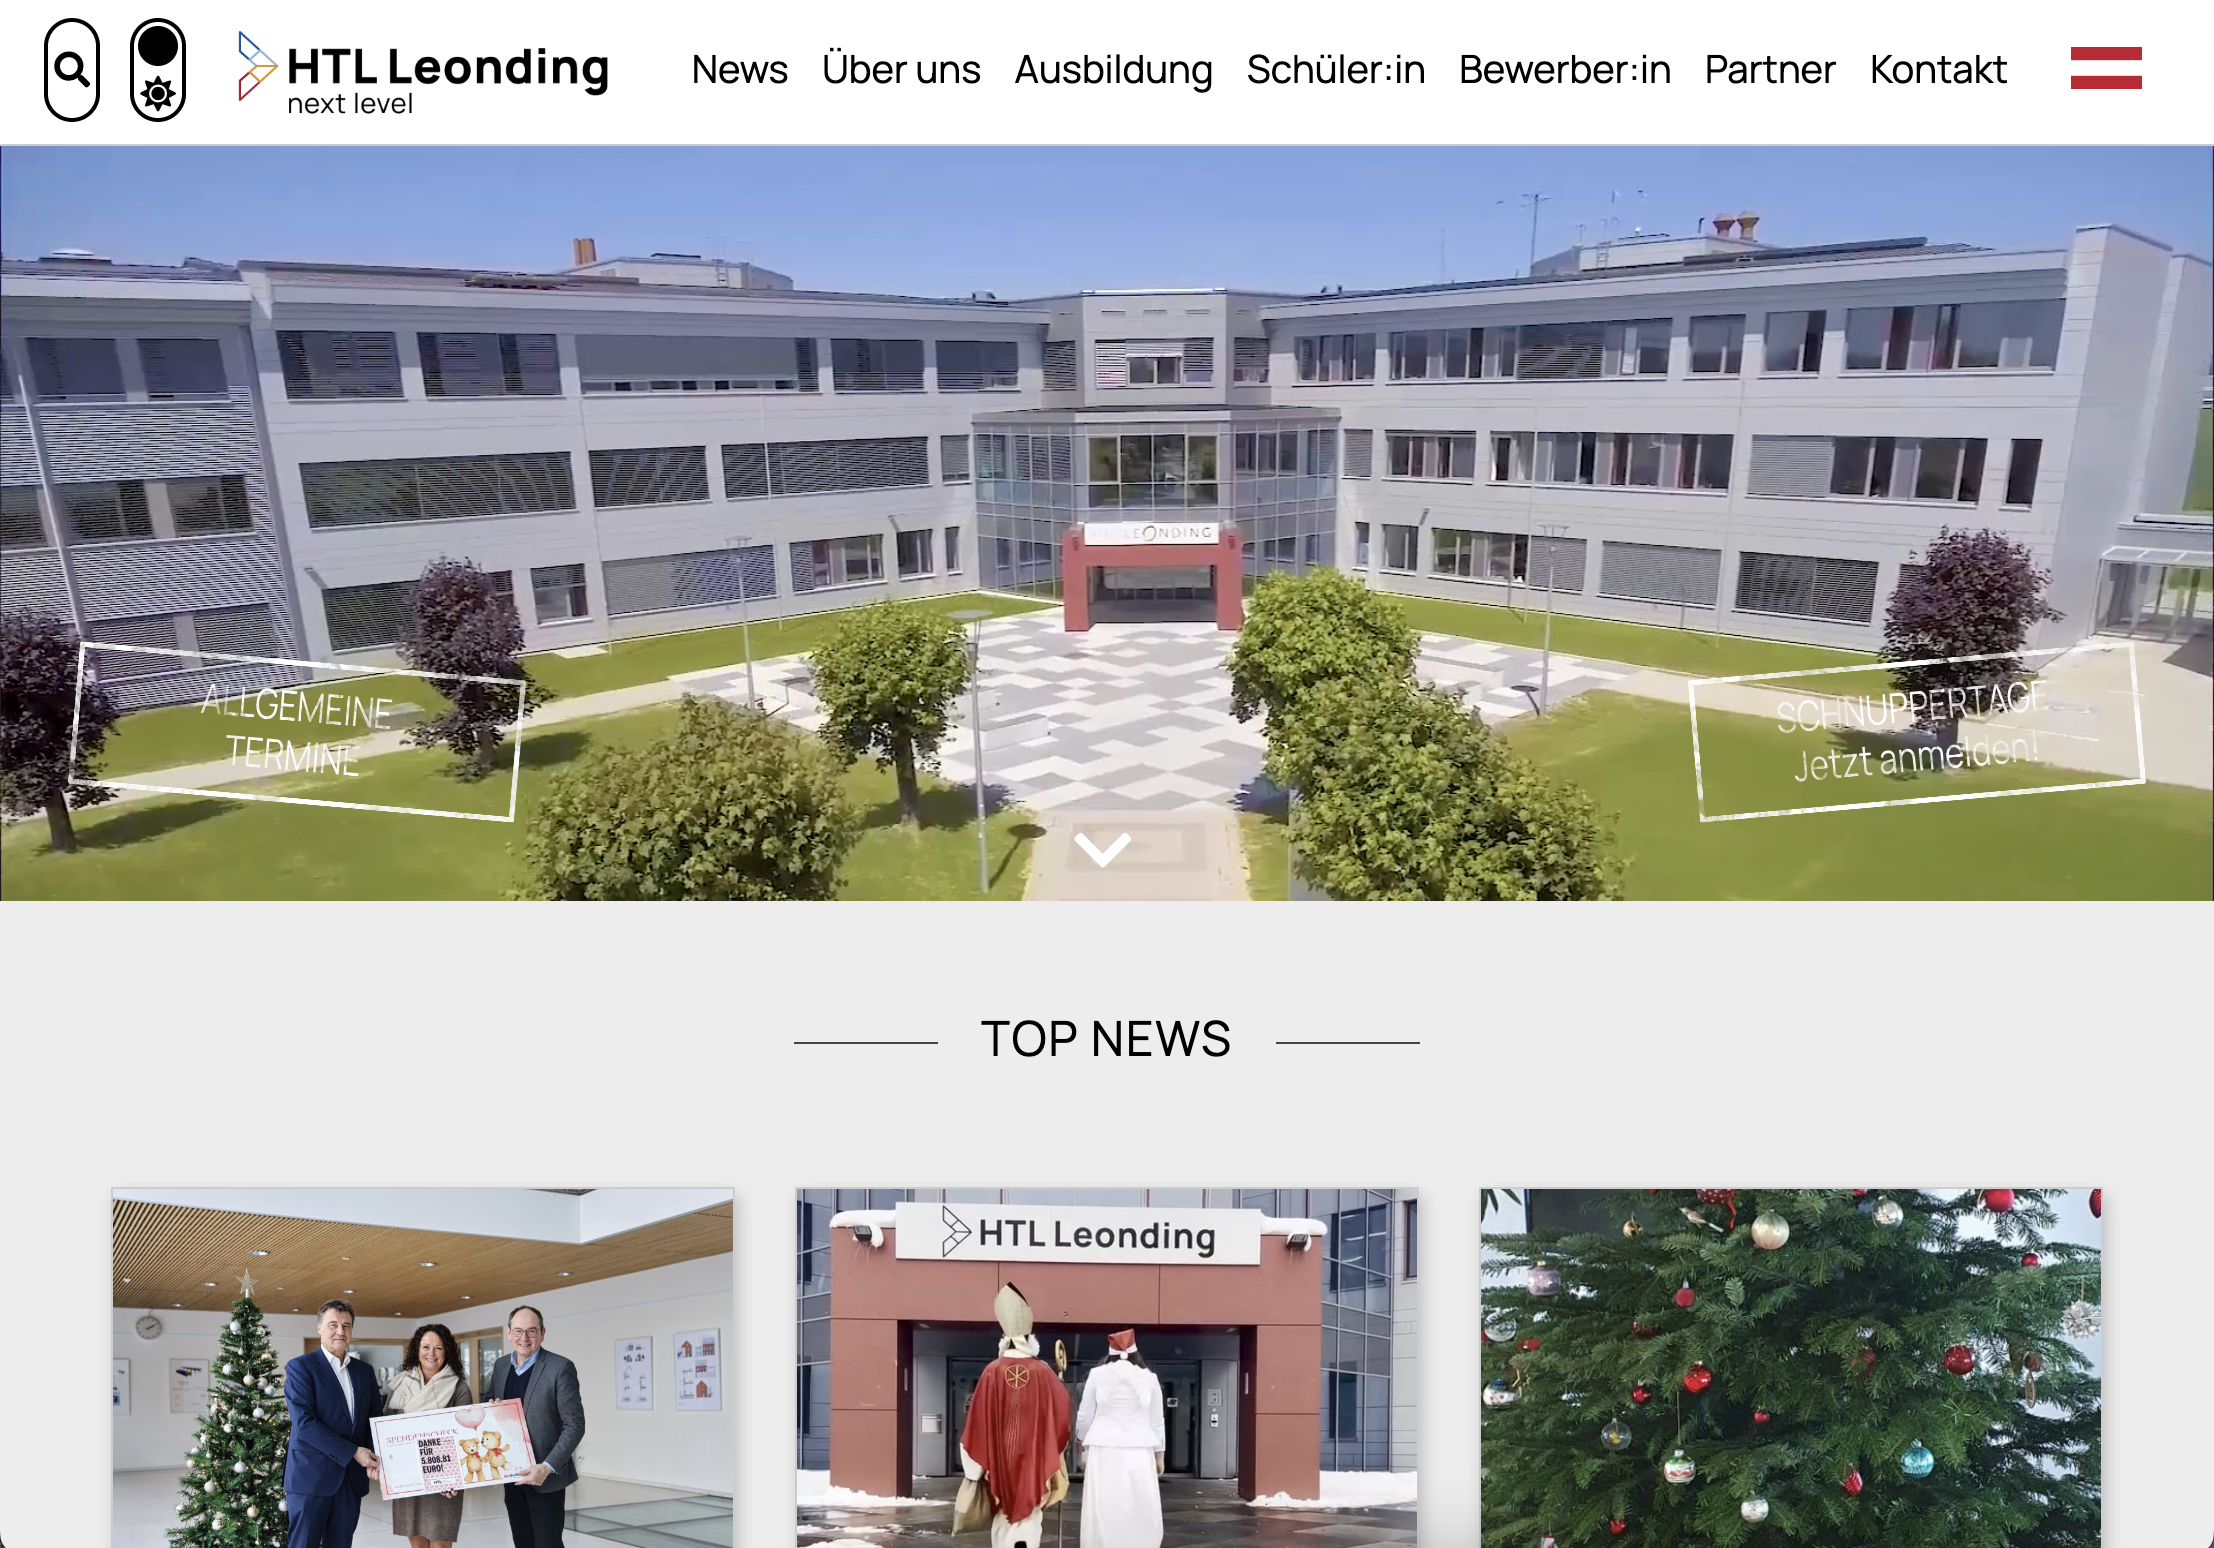
\includegraphics[scale=0.3]{pics/startseite_ausgangslage.png}
    \caption{Startseite Ausgangssituation}
    \label{fig:impl:startseite_ausgangslage}
\end{figure}


\section{Problemstellung}
\setauthor{Angerer Mona}
Die HTL Leonding-Website, die 2019 von Schülern auf Wordpress-Basis entwickelt wurde, 
zeigt eine durchaus den Anforderungen einer Schulhomepage entsprechenden, 
jedoch in die Jahre gekommene Plattform. Die technischen Möglichkeiten und Designstandards haben 
sich in den letzten Jahren erheblich weiterentwickelt, was dazu führt, dass die aktuelle 
Website nicht mehr den zeitgemäßen Ansprüchen entspricht. 

Die bestehende Website weist Unstimmigkeiten in der Benutzerführung auf, 
insbesondere im Hinblick auf die Menüstruktur, die als unübersichtlich wahrgenommen wird. 
UserInnenn fällt es schwer, sich auf der Oberfläche zurechtzufinden und den gesuchten Inhalt auf Anhieb zu finden. 
Während mancher Content nur schwer zu finden ist, weist die Homepage auch Inhalte auf, 
die an mehreren Stellen und unterschiedlichen Unterseiten zu finden sind. Dies verstärkt zusätzlich 
die Verwirrung und schlechte intuitive Handhabung. Zudem verfügt sie über lange Ladezeiten, was die 
Benutzererfahrung deutlich beeinträchtigt. Durch die langen Unterbrechungen, 
die in der Bedienung entstehen könnten und die immer kürzer werdende Aufmerksamkeitsspanne und Ungeduld der Menschen, 
könnte es nicht nur zu einer getrübten Stimmung, sondern sogar zum Verlassen der Website kommen. Das Design erscheint 
zu bunt und durch die vielen Bilder Videos, die oftmals einen Großteil der Seite einnehmen, 
wirkt der Webauftritt der HTL Leonding überladen und nicht mehr zeitgemäß. Des Weiteren folgt die Webanwendung einem strikten
Box-Design, was fehlende Dynamik zur Folge hat und eintönig wirkt. Auch im Mobile-Modus gibt es zudem Herausforderungen,
wie schwierige Bedienung des Menüs und Schwierigkeiten beim Zurechtfinden und Navigieren. Da immer mehr Menschen eher auf 
ihren Mobilgeräten und nicht nur auf ihren PCs und Laptops Webseiten aufrufen, gewinnt insbesondere dies progressiv an Bedeutung.

Es hat sich gezeigt, dass die Website möglicherweise nicht mehr effektiv die Bedürfnisse und 
Ziele der verschiedenen Nutzergruppen erfüllt. Die Schulleitung hat angesichts dieser Erkenntnisse den Vorschlag gemacht, 
im Rahmen einer Diplomarbeit einen neuen Webauftritt zu gestalten. Dies bietet die Chance, die bestehenden 
Herausforderungen zu adressieren, die Website zu modernisieren und eine verbesserte Benutzererfahrung für alle Zielgruppen zu schaffen.


\section{Aufgabenstellung und Ziele}
\setauthor{Angerer Mona}
Um ein breites Spektrum an Technologien abzudecken und unterschiedliche Ansätze zu fördern, werden zwei Teams mit dieser Diplomarbeit betraut. 
Diese Herangehensweise ermöglicht es, verschiedene Ideen und Lösungsansätze zu erforschen und so eine fundierte Grundlage für die Gestaltung 
des neuen Webauftritts der HTL Leonding zu schaffen.

Die Vorgabe besteht darin, als Backend das headless CMS Storyblok zu verwenden. Die Motivation hinter dieser Entscheidung 
liegt in der aktuellen Relevanz und Flexibilität dieses Content Management Systems. Die SchülerInnen werden dazu ermutigt, 
sich eingehend über verschiedene Frontend-Varianten zu informieren und dazu zu recherchieren, um diejenige zu finden, 
die sich am besten mit Storyblok kombinieren lässt und den Anforderungen am besten gerecht wird.
Die neue Website soll eine mit entsprechender Backend-Struktur aufgebaut sein, so dass
sie für die Zukunft eine leichte Wartung ermöglicht. 
Um die Benutzerfreundlichkeit zu erhöhen wird gefordert, den Content besser zu strukturieren,
abzuwägen, welche Inhalte ins LeoWiki ausgelagert werden sollen und die Inhalte so zu 
platzieren, dass eine intuivtive Navigation für alle Benutzergruppen ermöglicht wird.
Das Design der Website soll an die derzeitigen Standards und Trends angepasst werden
und mithilfe von Animationen und spannendem Design einladend und ansprechend gestaltet werden.

Das endgültige Ziel ist eine technisch sauber gelöste, gut strukturierte, ansprechend gestaltete
Weboberfläche, die eine einfache und intuitive Navigation ermöglicht. Alle relevanten Inhalte, die die HTL Leonding repräsentieren,
sind auf der Homepage zu finden und bilden ein einladendes Bild der HTL Leonding. 